\section{Expanding the Model for Effectiveness}

The Large Evaporative Cooler was the unique minimax choice at all 12 venues in the comfort benchmark. It had the lowest modeled hot-discomfort loss outright in 28 of 36 cases and tied for the lowest in the other eight.

Hot-discomfort loss counts SET degree-hours above $26\,^\circ\mathrm{C}$. In Boston's hot-dry case, the Large Evaporative Cooler produces $20.77\,^\circ\mathrm{C}$ SET and receives zero loss. The separate operating rule leaves cooling off when the baseline is already in the $23$--$26\,^\circ\mathrm{C}$ comfort band.

We compare each option's hot-discomfort loss with the lowest feasible loss in the same hour. We then select the option with the smallest maximum regret across the three weather cases, including no cooling in the comparison.

The baseline also puts the regret of the Fan in context. At Grove Hall, the largest shortfall with no cooling is 2.20 SET degree-hours, compared with 0.49 with the Fan. At Rosa Parks Plaza, the corresponding values are 2.56 and 1.78. The declines in maximum regret are about 1.71 and 0.78 SET degree-hours, respectively. Each of these comparisons uses the worst case for each option, which can occur in a different hour. Therefore, the difference between the two maxima describes how much installing the Fan reduces the worst shortfall across the three cases. A location with the larger baseline shortfall can gain less from the same upgrade. The site-level comparison helps identify where using only a fan would still leave a substantial gap between the available cooling and the best modeled outcome.

At Boston and Phoenix bus shelters, the Fan stays much closer to the best case than it does in Dallas. Its maximum regret is $0.49$ SET degree-hours at Grove Hall and $0.75$ at Central Avenue/Camelback, compared with $1.78$ at Rosa Parks Plaza. The hour that determines this gap also varies by site. Boston's gap occurs at peak temperature, while the hot-dry hour determines the maximum for the Dallas and Phoenix bus fans.

\begin{figure}[H]
    \centering
    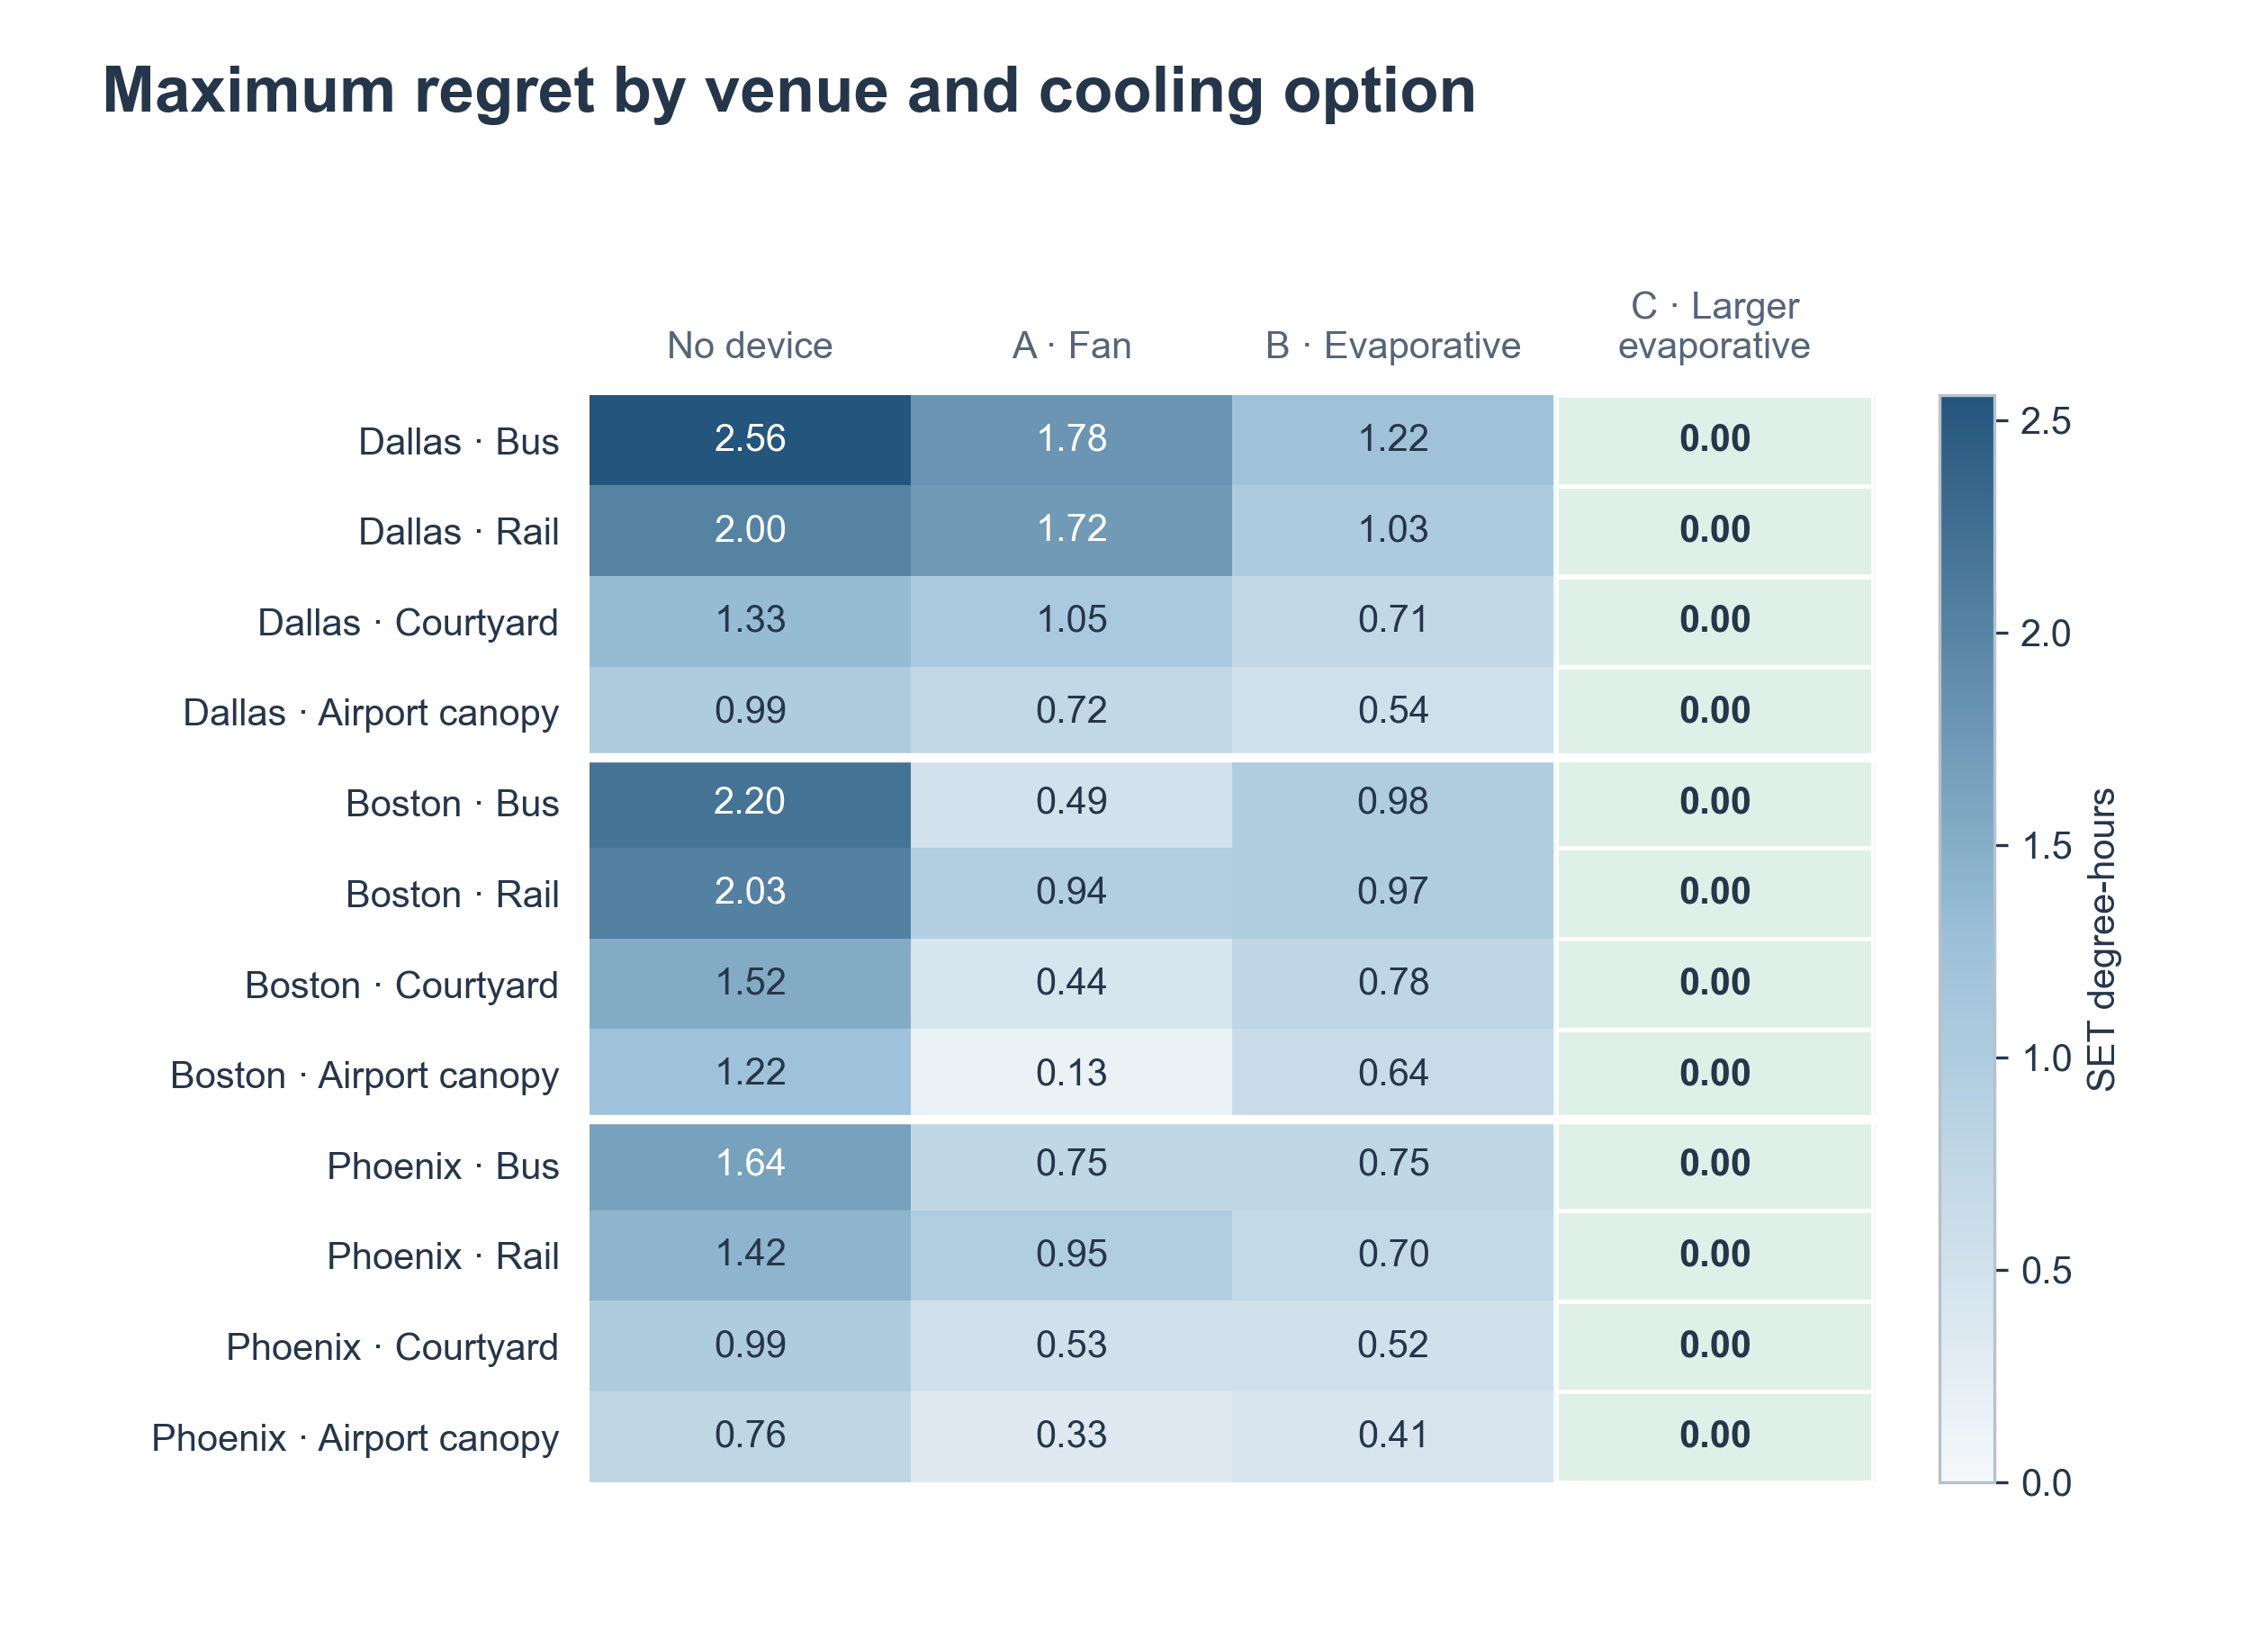
\includegraphics[width=0.88\linewidth,trim=0 0 0 69.12bp,clip]{Images/F7_maximum_regret_all_venues.png}
    \caption{Maximum regret in SET degree-hours across the three modeled scenarios. Green cells identify the comfort benchmark winner.}
    \label{fig:max-regret}
\end{figure}

At the Dallas bus shelter, maximum regret was 1.78 SET degree-hours for the Fan and 1.22 for the Small Evaporative Cooler. At the Dallas rail platform, the corresponding values were 1.72 and 1.03. The Large Evaporative Cooler had zero maximum regret at both sites.

In the comfort benchmark at Grove Hall, the Fan's maximum regret is about half that of the Small Evaporative Cooler ($0.49$ versus $0.98$ SET degree-hours). At the Phoenix bus shelter, both options round to $0.75$, so the Fan gives nearly identical worst-case regret with lower electricity use and zero evaporation. At the Phoenix rail platform, the Small Evaporative Cooler reduces the maximum regret from $0.95$ to $0.70$. Venue-level airflow therefore matters even when nearby sites share the same weather inputs.

Absolute comfort tells a second part of the story. At the Phoenix bus shelter, the Large Evaporative Cooler leaves peak-hour SET at $33.68\,^\circ\mathrm{C}$, almost $8\,^\circ\mathrm{C}$ above the comparison target. Its zero regret reflects its lead among the tested options. The remaining heat discomfort is still substantial.

\subsection{Resource Tradeoffs at Bus Shelters}

The Dallas bus and rail radars share the same axis scales. Both sites use the same equipment and share city weather, so their modeled resource inputs coincide. The different regret profiles reflect how those devices perform under each venue's airflow assumptions. For Dallas at peak temperature, the added relief from switching from the Fan to the Large Evaporative Cooler is about $1.22\,^{\circ}\mathrm{C}$ of SET at the bus shelter and $1.20\,^{\circ}\mathrm{C}$ at the rail platform. The extra electricity is $2.25$ kWh at either site. Across the three scenarios, the Small Evaporative Cooler's maximum regret is $1.22$ at the bus shelter and $1.03$ at the platform. The similar peak-hour upgrades and different maximum regrets show why we compare the full set of weather cases. The shared radar scales make the size of the regret differences directly comparable between venues. On the resource spokes, the paths align because we use the same device specifications and outdoor weather within Dallas. Each spoke represents a separate outcome. We read the regret spoke first to identify the minimax choice, then read the other spokes to see what it takes to achieve that result in purchase cost, electricity, and evaporated water.

\begin{figure}[H]
    \centering
    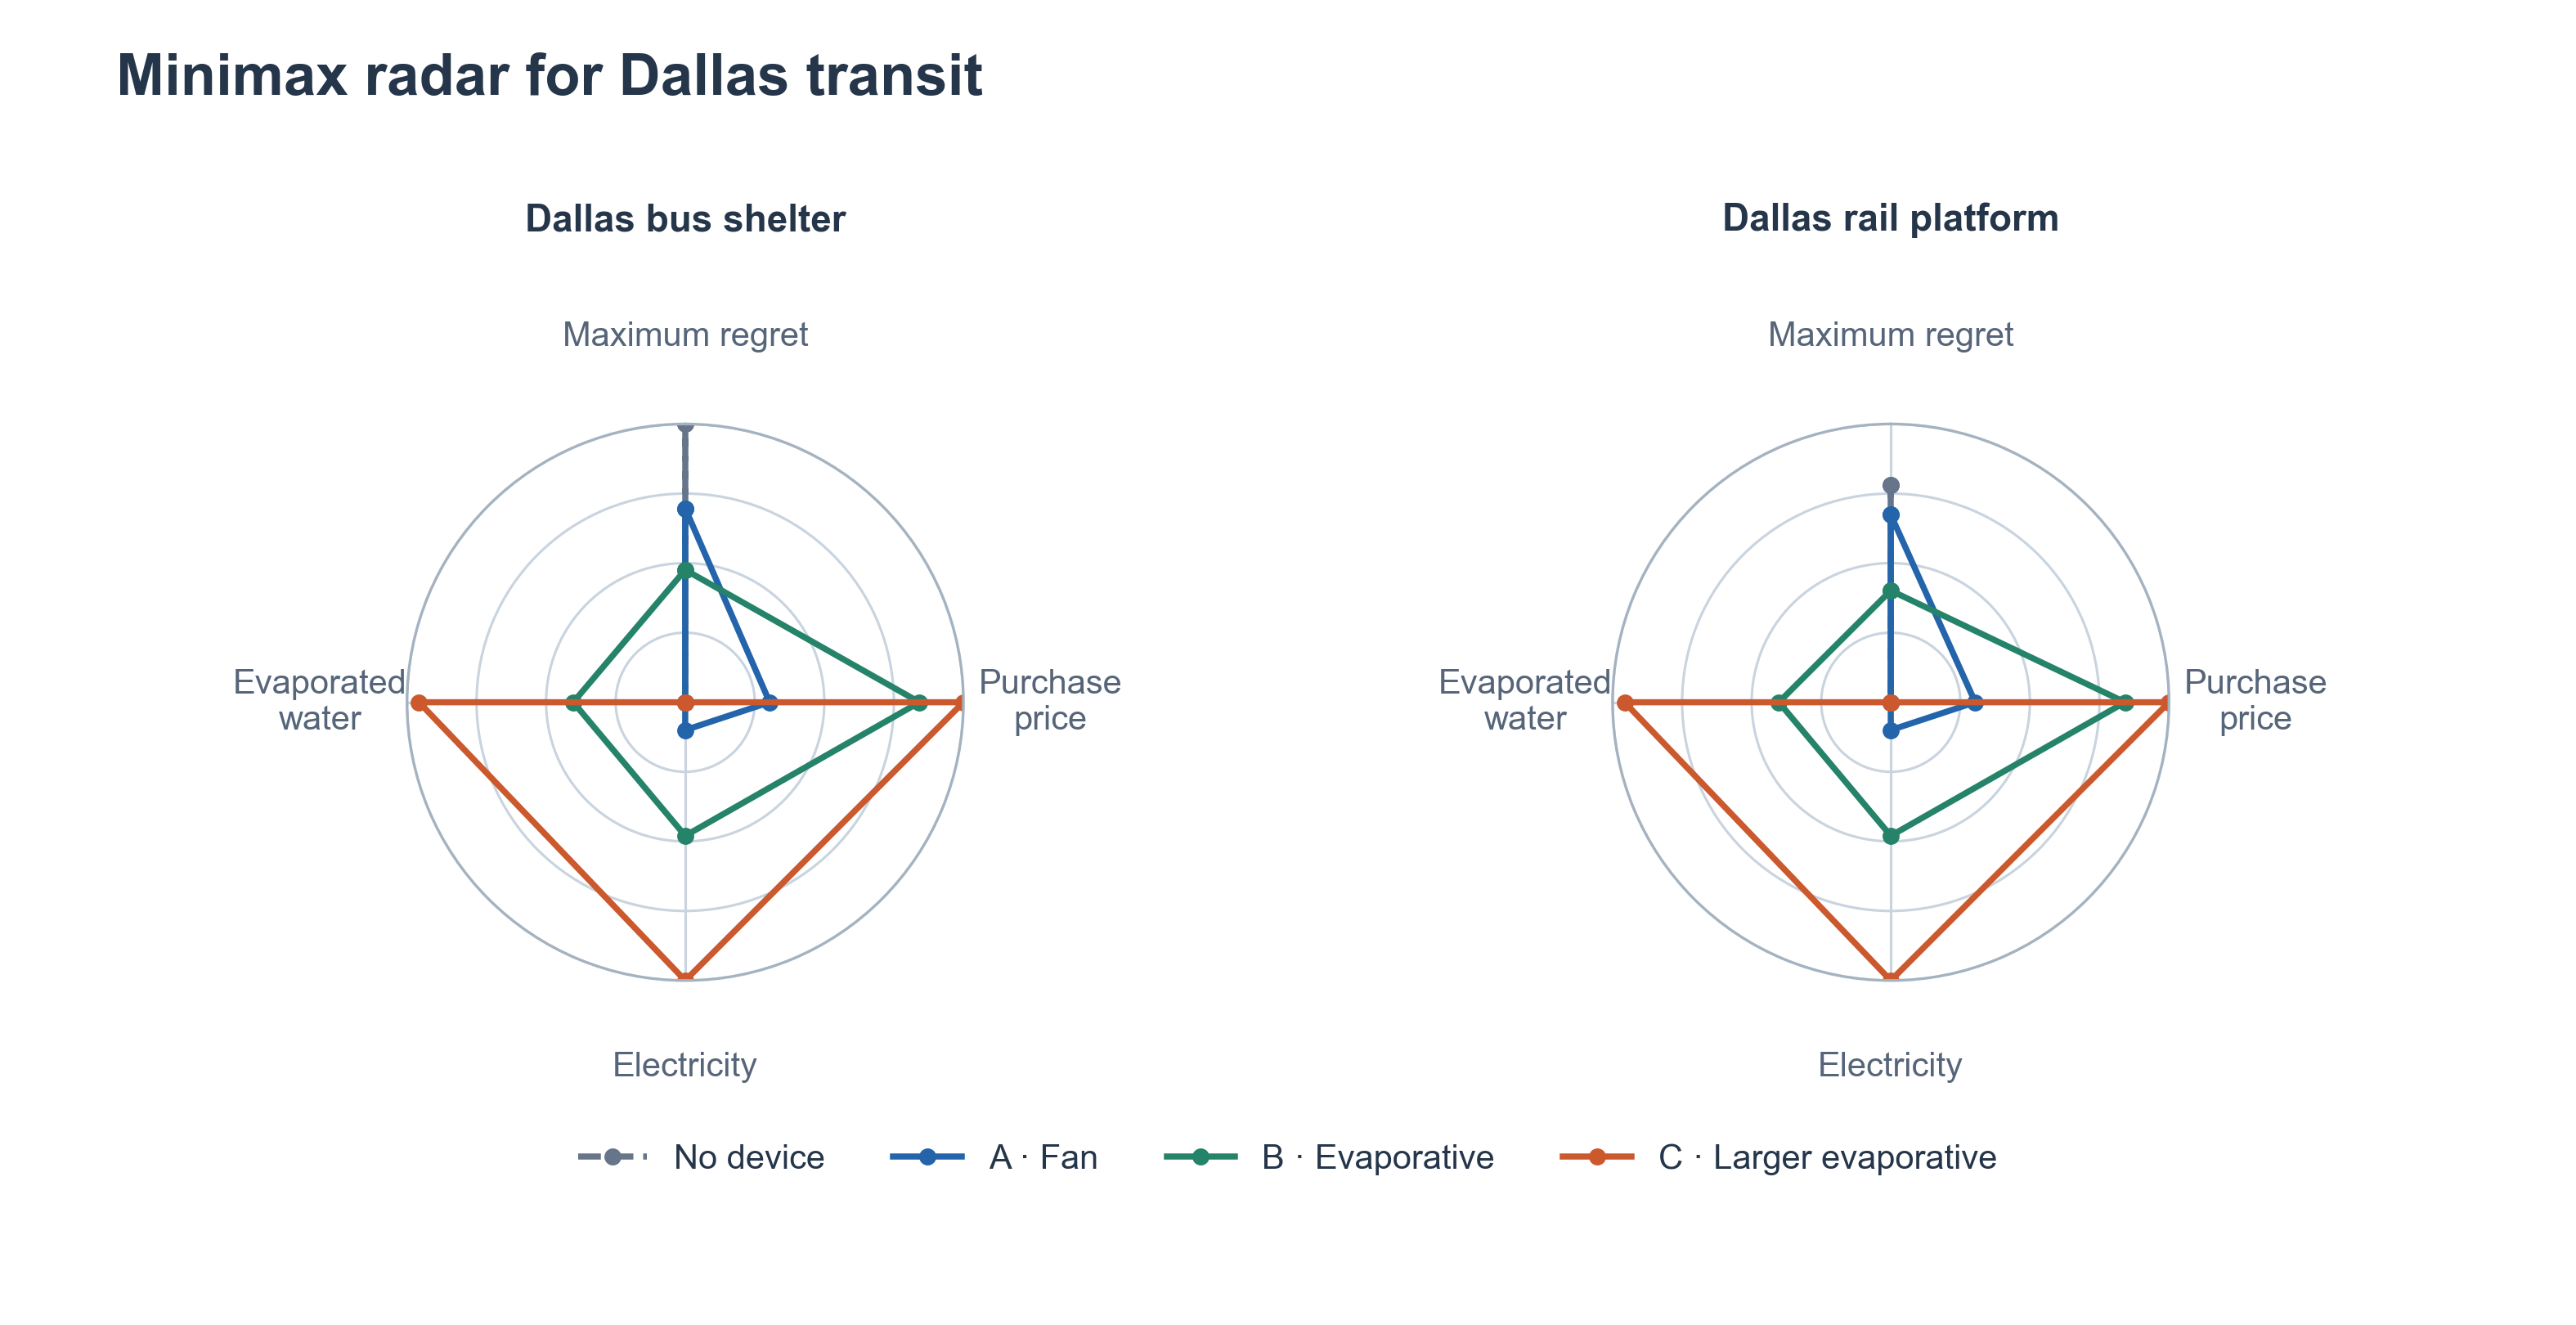
\includegraphics[width=0.94\linewidth,trim=0 0 0 51.36bp,clip]{Images/F15_dallas_transit_minimax_radar.png}
    \caption{Dallas bus shelter and rail platform radars with common scales for both venues. Minimax selection uses the maximum-regret axis.}
    \label{fig:dallas-radar}
\end{figure}

The Large Evaporative Cooler has a recorded reference purchase price of \$4,939~\cite{portacool_4000}. It draws 2.50 kWh over the modeled hour, and evaporates about 44 to 84 kg of water across the 36 modeled cases. Among bus shelters, the Small Evaporative Cooler is on the cost--regret frontier in Dallas. In Boston and Phoenix, the Fan costs less and has lower maximum regret than the Small Evaporative Cooler.

\begin{figure}[H]
    \centering
    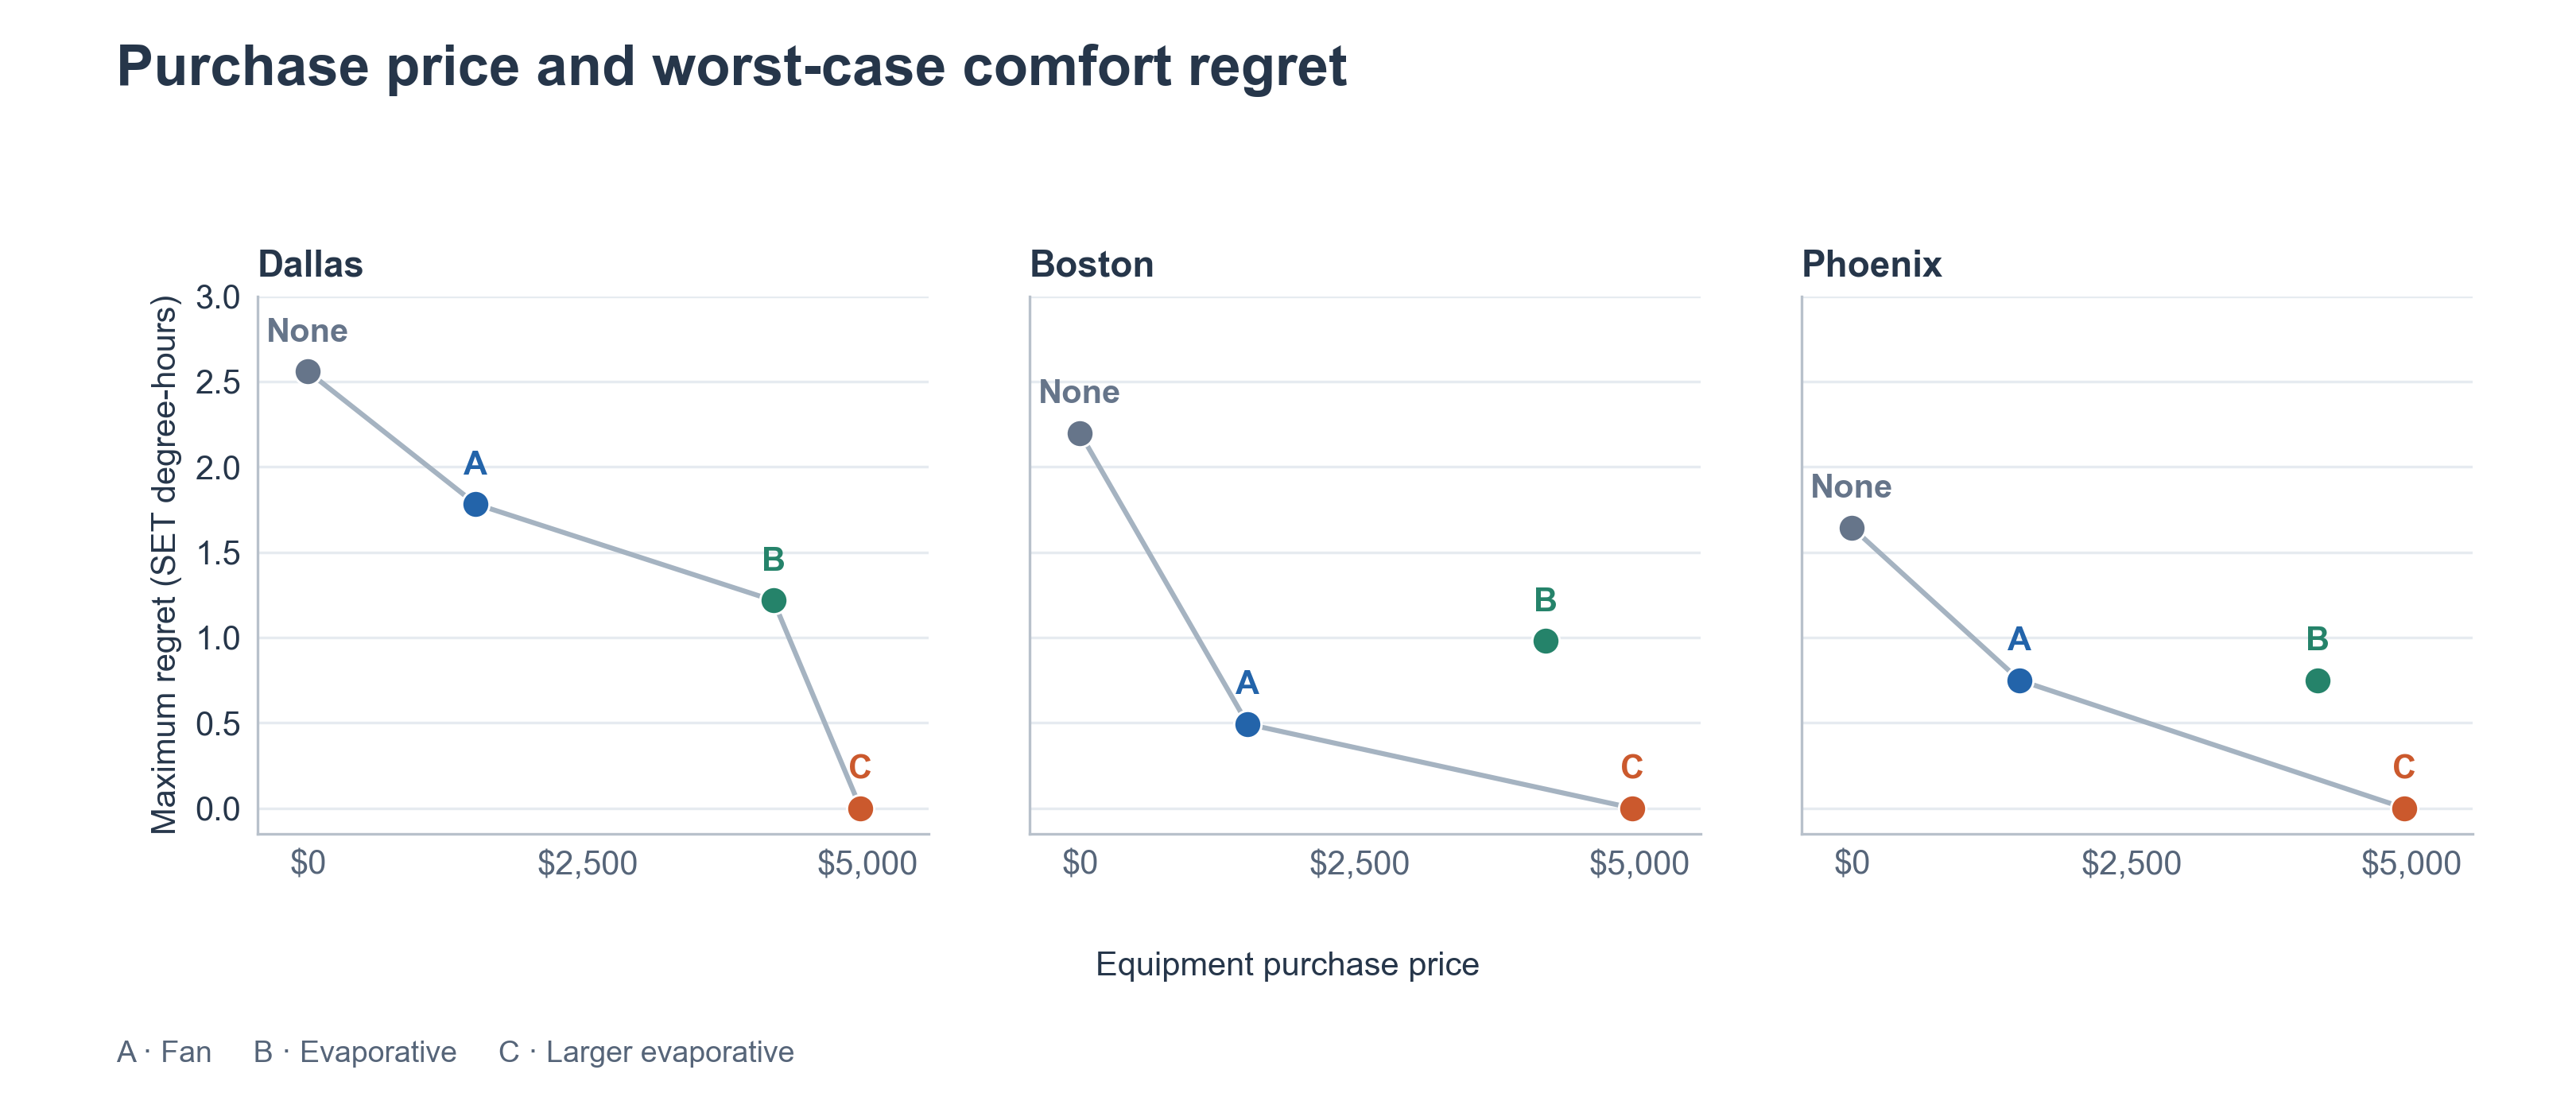
\includegraphics[width=0.92\linewidth,trim=0 0 0 68.40bp,clip]{Images/F13_bus_cost_regret_frontier.png}
    \caption{Purchase price and maximum regret at the three bus shelters. The frontier connects options for which a lower-regret choice costs more.}
    \label{fig:cost-regret}
\end{figure}

The curves also show how the value of upgrading varies across cities. In Dallas, upgrading from the Fan to the Small Evaporative Cooler costs \$2,660 and reduces maximum regret by about $0.56$ SET degree-hours. The Large Evaporative Cooler costs another \$780 and removes the remaining $1.22$ degree-hours of regret, alongside higher one-hour electricity and water use. In Phoenix, the Fan and Small Evaporative Cooler have nearly identical regret. In Boston, the Fan has lower regret and costs \$2,660 less than the Small Evaporative Cooler. These examples identify where the middle option merits a closer look and where the Fan already captures most of the attainable benefit.


\subsection{Remaining Discomfort and Sensitivity}

With the Large Evaporative Cooler, peak-hour SET ranged from 28.12\ensuremath{^{\circ}\mathrm{C}} to 33.98\ensuremath{^{\circ}\mathrm{C}} across the 12 venues. Every modeled peak-hour result remained above the 26\ensuremath{^{\circ}\mathrm{C}} comparison target.

\begin{figure}[H]
    \centering
    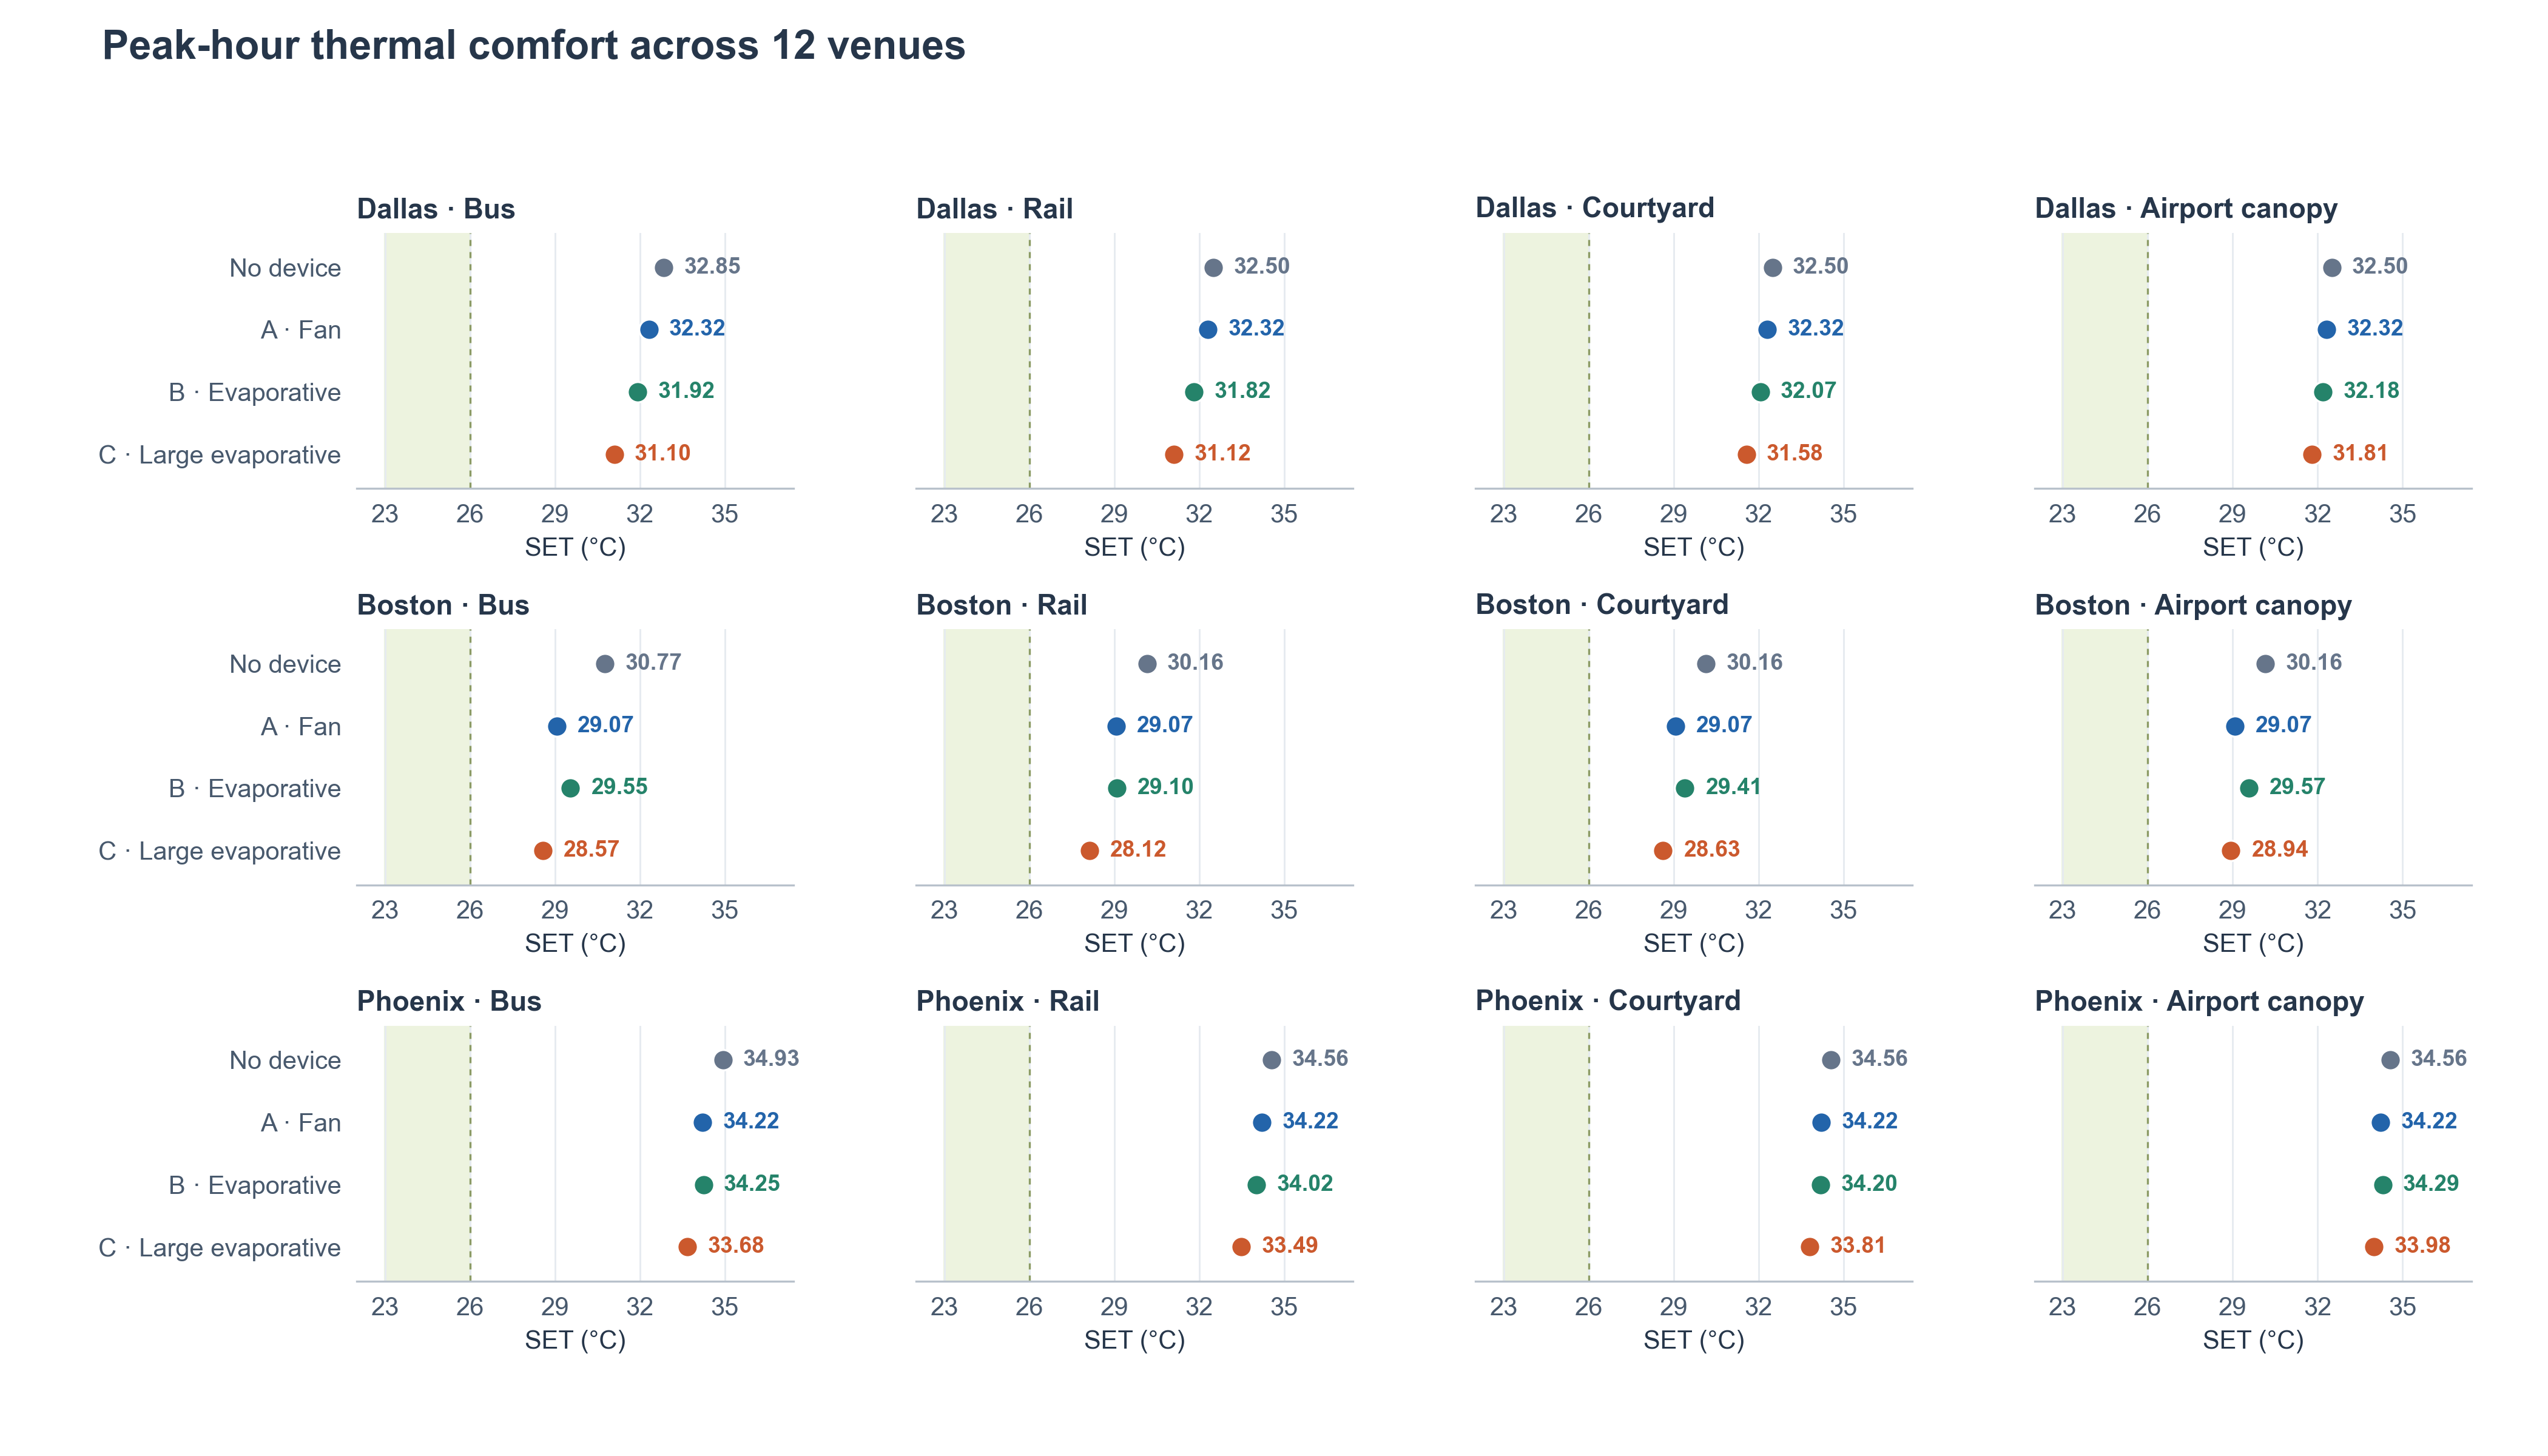
\includegraphics[width=0.95\linewidth,trim=0 0 0 69.84bp,clip]{Images/F3_all_venues_peak_comfort.png}
    \caption{Peak-hour SET at all 12 venues. The shaded band marks the 23--26\ensuremath{^{\circ}\mathrm{C}} comparison target.}
    \label{fig:peak-comfort}
\end{figure}

We varied one input at a time over five evenly spaced settings from $95\%$ to $105\%$ of its baseline in the recorded units. We tested bounded weather, airflow, equipment, exposure, and occupant inputs. The lower and upper SET thresholds were swept separately over $21.85$--$24.15\,^\circ\mathrm{C}$ and $24.70$--$27.30\,^\circ\mathrm{C}$. Other independent inputs stayed at baseline. Inflow and outflow changed together to preserve mass balance, and the radiant-temperature proxy followed outdoor temperature. We recomputed the minimax choice across the three scenarios at each setting.

\begin{figure}[H]
    \centering
    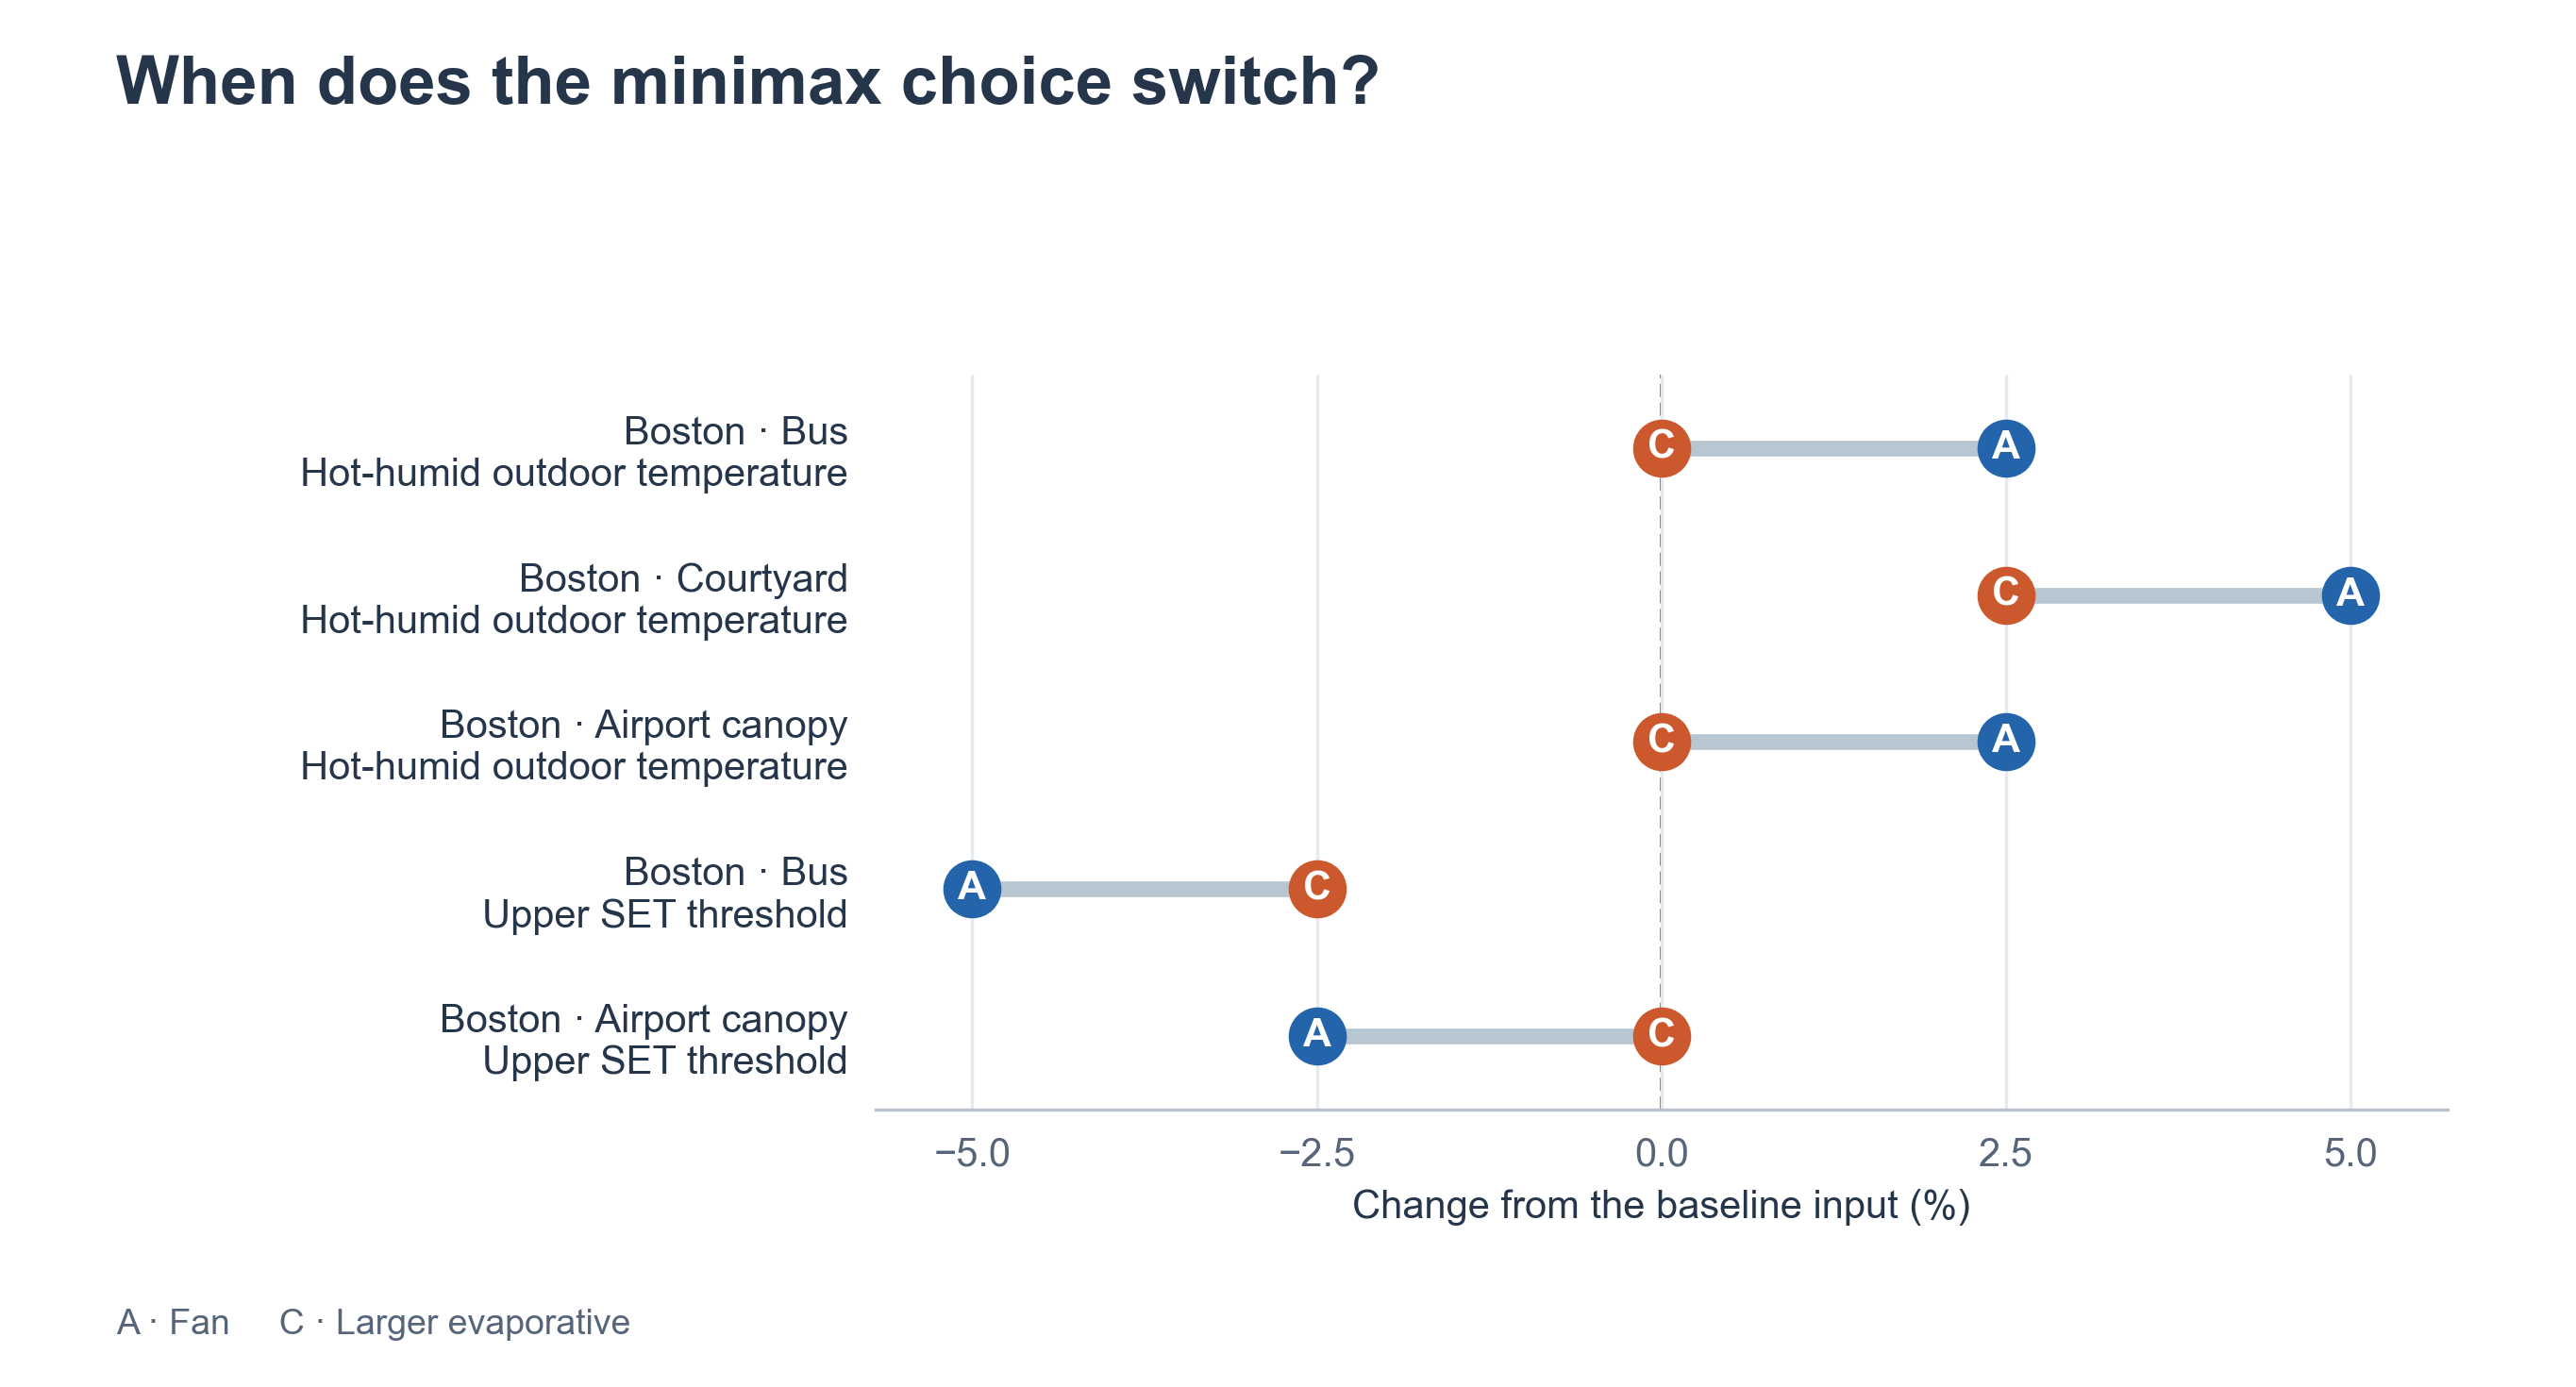
\includegraphics[width=0.78\linewidth,trim=0 0 0 94.80bp,clip]{Images/F14_minimax_sensitivity_switches.png}
    \caption{Five Boston switching intervals. Endpoints are adjacent tested settings with different minimax choices.}
    \label{fig:regret-switches}
\end{figure}

Increasing hot-humid outdoor temperature shifted the Boston choice from the Large Evaporative Cooler to the Fan between $30.39$ and $31.15\,^\circ\mathrm{C}$ at Grove Hall and the airport canopy, and between $31.15$ and $31.91\,^\circ\mathrm{C}$ at the courtyard. Raising the upper SET threshold shifted the choice from the Fan to the Large Evaporative Cooler between $24.70$ and $25.35\,^\circ\mathrm{C}$ at Grove Hall and between $25.35$ and $26.00\,^\circ\mathrm{C}$ at the airport canopy. These intervals bracket switches between sampled settings.
